\documentclass[12pt,a4paper]{article}
\usepackage[utf8]{inputenc}
\usepackage{amsmath}
\usepackage{amsfonts}
\usepackage{amssymb}
\usepackage{graphicx}
\usepackage{indentfirst}
\usepackage{hyperref}
\usepackage{booktabs}
\usepackage{longtable}
\usepackage{listings}
\usepackage{float}
\usepackage[left=2cm,right=2cm,top=2cm,bottom=2cm]{geometry}
\title{Laboratorio HTTP}
\author{Francisco Bolzan - Lucio Trincheri - Joel Torboli}

\begin{document}
	\maketitle
	\section{Introducción}
	Para comenzar, leímos la documentación de los slides sobre Webserver proveniente de la página de Netkit, así como el laboratorio y su configuración básica. Aquí aprendimos sobre la herramienta 'links' para acceder a un servidor web, así como la configuración del mismo y los archivos necesarios. Esto nos permitió especular como sería el funcionamiento si el laboratorio fuese ampliado, pero como no había más documentación que leer, proseguimos al desarrollo de las actividades solicitadas.
	\section{Envio de datos}
	Como primer paso, creamos un archivo 'index.html', el cual posee la simple función de enlazar a 2 formularios; uno que envía los datos a través de GET y otro mediante POST.
	Tras esto activamos la captura de tramas con el siguiente comando: 
	
	\verb|tcpdump -w /hosthome/'captura'.pcap -s 0| 
	
	Finalizado esto, mediante 'links' ingresamos al servidor mediante su IP, donde completamos el formulario (Tanto mediante POST como GET).
	
	Una vez realizado el paso anterior, estas tramas fueron analizadas con WireShark, donde nos centramos en buscar las diferencias entre GET y POST y su funcionamiento.
	
	Al analizar el envío de datos a nivel de protocolo, nos dimos cuenta que GET envía los mismo a traves de la URL de la página, situación que puede llegar a ser indeseable cuando se trabaja con información privada o personal, tal como contraseñas, tarjetas de credito, etc. Por su parte, POST enviá los datos como un paquete 'oculto', por lo que si alguien captura la URL del usuario, no podrá extraer ninguna información de esta misma.
	
	\begin{figure}[H]
		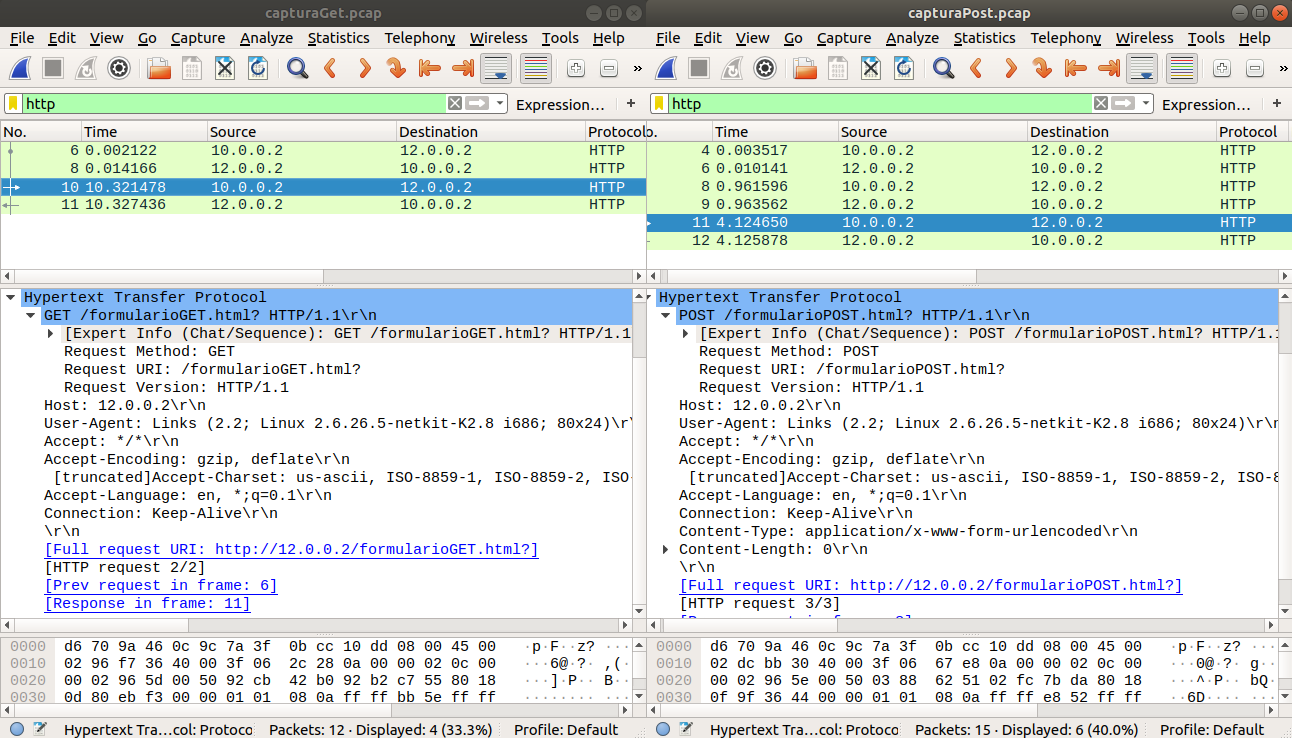
\includegraphics[width=\linewidth]{getvspost.png}
		\caption{Captura de tramas HTTP}
		\label{fig:img1}
	\end{figure}

	En la figura 1 se puede observar las tramas en donde se enviaron los formularios mediante HTTP. Del lado izquierdo se muestra la informacion de la trama con el formulario que emplea el metodo GET, se observa que este trabaja sin condificar la informacion, es decir, envia el formulario en forma de URL. Mientras que en el lado derecho donde se observa la trama con el formulario que emplea el metodo POST, este define:
	
	\verb| Content-type: application/x-www-form-urlencoded\r\n|
	
	De esta definicion se deduce que el metodo POST codifica la infomacion del formulario en forma de un string.
	
	\section{Persistencia}
	HTTP 1.1 es persistente ya que utiliza TCP para mantener una pseudo sesión por la cual se envían y reciben los paquetes. El tiempo de dicha conexión esta dictado por apache, normalmente van de 15 a 5 segundos, lo que permite que durante estas ventanas de conexión múltiples paquetes sean enviados/recibidos pero tampoco saturan al servidor con muchas conexiones constantes y paralelas.
	
	\begin{figure}[H]
		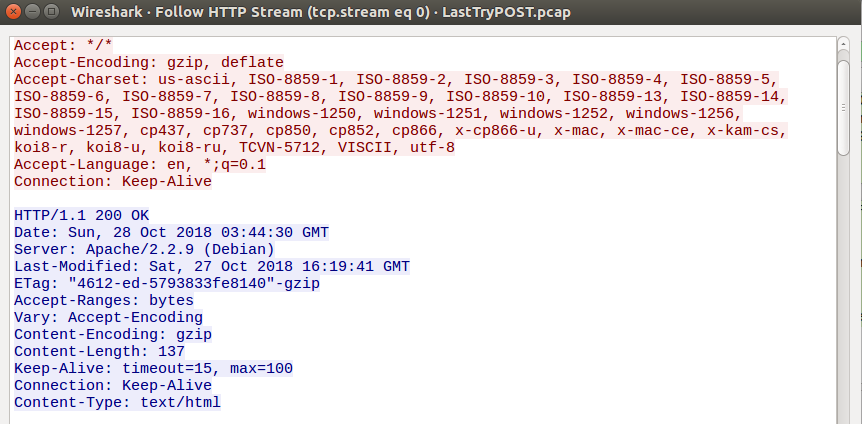
\includegraphics[width=\linewidth]{crop.png}
		\caption{Persistencia en HTTP}
		\label{fig:img2}
	\end{figure}
	
	Como se observa en la figura anterior, la conexión tiene la característica de mantenerse viva tras el envío del paquete, indicando un timeout para esta de 15 segundos.
	\section{DNS y WWW}
	La WWW necesita del DNS para iniciar el proceso de enrutamiento, en el cual, utilizando un buscador se introduce una URL la cual DNS asocia con su respectiva IP de servidor, HTTP luego procesa el resto del enrutamiento para asi obtener al principio el HTML básico de la pagina y luego pedir el resto de paquetes necesarios.
	
	Para lograr esto, el laboratorio fue configurado de la siguiente manera.
	
	\section{Configuracion}
	La configuración de los subdominios y sus alias fue realizada en el router de la red, actuando este a su vez como NS. Aquí asignamos los nombres (subdominios)  "www.tec" al primer servidor con IP 11.0.0.1 y "www.mit" al segundo con IP 12.0.0.2.
	
	Tras esto, con el cliente intentamos acceder al servidor, solo que, esta vez ingresamos "www.tec.net" en la búsqueda de links, al contrario de su IP.
	Este intento fue satisfactorio, con lo que comprobamos que el NS fue correctamente configurado.
	
	
	\section{Apache}
	
	Finalmente, para la última actividad modificamos los DNS para que apunten a uno solo de los servidores y que el redireccionamiento quede a cargo de Apache.
	Para esto lo primero fue modificar los archivos DNS, solo fue necesario cambiar la IP de algún servidor por la del otro y listo.
	Para que Apache reconociese a ambos servidores individualmente primero creamos dos directorios, uno para cada servidor con paginas distintas dentro de cada uno.
	Buscando un poco sobre las opciones y configuracion de Apache descubrimos que el mismo posee una carpeta de sitios disponibles dentro de la cual estan los .conf de dichas páginas, con esto pudimos modificar dichos archivos para que cada uno supiese el nombre de su servidor, el alias y donde buscar la pagina del mismo.
	Una vez hecho esto con ambos servidores desactivamos los sitiso "default" de Apache con --a2dissite default (en /etc/apache2/sites-available)--, luego activamos los nuestros con a2ensite, reiniciamos Apache y comprobamos satisfactoriamente el resultado. 
\end{document}